\documentclass[a4paper,12pt]{article}
\usepackage{../styledoc19}


\begin{document} % конец преамбулы, начало документа
	\year{2019}
	\itsHSE
	\academicTeacher{Преподаватель департамента \vfill программной инженерии  факультета компьютерных наук}
	{М. К. Горденко}
	
	\projectName{IOS-ПРИЛОЖЕНИЕ <<СОЦИАЛЬНАЯ СЕТЬ ДЛЯ СОТРУДНИКОВ НИУ ВШЭ>>}
	
	\titleList{Пояснительная записка}{RU.17701729.04.03-01 81 01-1-ЛУ}
	\par\vspace{60mm}
	\nameOfAuthor{БПИ174}{Д. Ю. Редникина}
	\tabForFirstPage
	
						\newpage
	
	\pagestyle{fancy}
	\lhead{УТВЕРЖДЕН \newline
	 	RU.17701729.04.03-01 81 01-1-ЛУ}
	\vspace*{\fill}
	\begingroup
	\centering
	\tabForFirstPage
	\projectName{IOS-ПРИЛОЖЕНИЕ <<СОЦИАЛЬНАЯ СЕТЬ ДЛЯ СОТРУДНИКОВ НИУ ВШЭ>>}
	\titleList{Пояснительная записка}{RU.17701729.04.03-01 81 01-1-ЛУ}
	\listNumber{54}
	
	\endgroup
	\vspace*{\fill}
	
	
						\newpage
	\lhead{ }
	\chead{\vfill \thepage \vfill  RU.17701729.04.03-01 81 01-1-ЛУ}
	\rhead{ }
	\cfoot{ }
	%delete this if you are not writing a TZ
	\cfoot{\tabForTZ}
	\tableofcontents
	\newpage
	\section{Введение}
	\subsection{Наименование программы}
	\subsubsection{Наименование программы на русском языке}
iOS-приложение <<Социальная сеть для сотрудников НИУ ВШЭ>>
\subsubsection{Наименование программы на английском языке}
iOS application <<Social network for HSE staff>>
	\subsection{Документы, на основании которых ведется разработка}
	\begin{enumerate}
		\item  Приказ декана факультета компьютерных наук Национального Исследовательского университета <<Высшая школа экономики>> № 2.3-02/1012-0 2 от 10.12.18.
		\item Техническое задание <<iOS-приложение <<Социальная сеть для сотрудников НИУ ВШЭ>>.
	\end{enumerate}
	\newpage
	\section{Назначение и область применения}
	% \subsection{Назначение программы }
	\subsection{Функциональное назначение}
	Программа применяется как средство коммуникации между сотрудниками НИУ ВШЭ. Сервис также позволяет сотрудникам НИУ ВШЭ координировать совместные исследования и проекты научного характера. Приложение предоставляет доступ к общению посредством сообщений, дает возможность делиться новостями с помощью публикации постов. Также приложение дает возможность фильтровать новости по интересущим темам. 

	\subsection{Эксплуатационное назначение}
	% ЭКСПЛУАТАЦИОННОЕ НАЗНАЧЕНИЕ

Программа будет использоваться как средство общения и огранизации работы над совместными научными проектами между сотрудниками с одного или разных направлений/ факультетов/ кампусов. 


Таким образом, программный продукт позволит решить проблему коммуникации между факультетами, кампусами НИУ ВШЭ и даст возможность наладить взаимодействие между преподавателями университета, будет способствовать развитию научной деятельности между разными факультетами и кампусами.
	\subsection{Область применения}
	% ОБЛАСТЬ ПРИМЕНЕНИЯ

НИУ ВШЭ очень большой вуз с кампусами в разных городах России. Преподавателям сложно общаться между собой, узнавать последние новости, связанные с написанием статей, научно-исследовательской деятельностью коллег. Разрабатываемая программа позволит наладить взаимодействие преподавателей и будет способствовать развитию научной деятельности и коммуникации между факультетами и кампусами университета.

Задача социальной сети заключается в обеспечении коммуникации, обмене актуальной научной и общеуниверситетской информацией, знакомстве научных работников и преподавателей с разных факультетов и кампусов. 

Разрабатываемая программа является прекрасной площадкой для начала исследований, обсуждения научных работ, общения по научным и университетским тематикам для сотрудников университета НИУ ВШЭ.
	
					\newpage 
	\section{Технические характеристики}
	\subsection{Постановка задачи на разработку программы}
	
	
		% требования
% dyurednikina
% version 1.2
% last modified 7.05.2019


Программа выполняется в рамках темы курсовой работы в соответствии с учебным планом подготовки бакалавров по направлению 09.03.04 «Программная инженерия» Национального исследовательского университета «Высшая школа экономики», факультет компьютерных наук.

Разработка требований велась совместно с командой и заказчиком в рамках предмета <<Групповая динамика и коммуникации в программной инженерии>>



\textit{Состав команды}:
\begin{itemize}
	\item Анна Михалева - android-developer;
	\item Константин Манежин - web-developer;
	\item Илья Костюченко - backend-developer;
	\item Дарья Редникина - iOS-developer;
\end{itemize}


\textit{Заказчик}:
\begin{itemize}
	\item Девятьярова Анна Дмитриевна, Факультет бизнеса и менеджмента/ 
	Кафедра управления человеческими ресурсами.
\end{itemize}
% \subsection{Клиентские приложения}
%\renewcommand{\labelenumi}{FR-\arabic{enumi})}
\renewcommand{\labelenumi}{\textbf{FR-\arabic{enumi}}.}

\renewcommand{\labelenumii}{\textbf{FR-\arabic{enumi}.\arabic{enumii}}.}

\renewcommand{\labelenumiii}{\arabic{enumiii}.}

\begin{enumerate}
	\item \textbf{Авторизация клиента\\}
	Чтобы использовать программу, клиент должен иметь возможность авторизоваться в системе.
	\begin{enumerate} \label{req: auth}
		\item При регистрации в социальной сети клиенту необходимо заполнить обязательные поля регистрации: \label{FR-1.2}
		\begin{enumerate}
			\item (\textit{Verified, автор: заказчик}) \\ФИО;
			\item (\textit{Verified, автор: заказчик}) \\Факультет;
			\item (\textit{Verified, автор: заказчик})\\Почта;
			\item (\textit{Verified, автор: заказчик})\\Должность; 
			\item (\textit{Verified, автор: заказчик})\\Город; 
		\end{enumerate}
		\item (\textit{Verified, автор: Илья})\\Уже зарегистрированный клиент для входа в социальную сеть должен ввести свою почту с доменом \verb+@hse.ru+.
		\item (\textit{Verified, автор: Анна})\\
		После успешной авторизациии/регистрации пользователю будет выслан код на введенную им почту, который нужно ввести в специальное поле в приложении, только после правильного ввода кода клиент сможет войти в социальную сеть.
	\end{enumerate}
	\item \textbf{Просмотр профиля пользователя}
	\begin{enumerate}
		\item (\textit{Verified, автор: Дарья})\\Должна быть возможность редактирования у пользователей выше перечисленных полей (см. требование \nameref{FR-1.2}), заполненых при регистрации, в настройках профиля. 
		\item (\textit{Verified, автор: команда, Анна})\\
		На странице профиля должна быть возможность просмотра раннее опубликованных постов человека. 
		\item (\textit{Verified, автор: Константин, заказчик})\\ 
		Также на странице должна быть возможность просмотра личных данных пользователя, то есть информации из требования \nameref{FR-1.2}
		\item (\textit{Verified, автор: Анна})\\
		На странице пользователя должна быть возможность написать сообщение пользователю в диалог.
		\item (\textit{Verified, автор: Анна})\\
		На странице пользователя должна быть возможность добавить пользователя в существующий канал.
	\end{enumerate}
	\item \textbf{Публикация постов\\} 
	Клиент имеет возможность опубликовать текстовую информацию от своего имени, чтобы она отображалась в ленте у других пользователей приложения и у него в профиле.
	\begin{enumerate}
		\item (\textit{Verified, автор: Илья})\\
		При написании поста у пользователя есть возможность добавить хэштеги к текстовой информации.
		\begin{enumerate}
			\item Хэштеги должны состоять из одного слова
			\item Хэштеги должны состоять из латинских и русских букв, допустимые символы при написании хэштега: нижнее подчеркивание, цифры.
			\item При неверном формате введенного хэштега он не будет опубликован вместе с написанным постом.
		\end{enumerate}
		\item (\textit{Verified, автор: Константин})\\
		При выборе хэштегов пользователю должны предлагаться autosuggested hashtags, раннее использованные в приложении другими пользователями при публикации постов.
		\item (\textit{Verified, автор: Анна})\\
		Должна быть поддержка разметки markdown, syntax highlighting при написании поста. 
		\item (\textit{Verified, автор: Дарья})\\
		При выходе из раздела создания поста, должна быть возможность сохранить черновик с текущем текстом и набором хэштегов. 
	\end{enumerate}
	\item \textbf{Лента\\}
	Пользователь должен имеет возможность, находясь в ленте, совершать поиск по интересущим его хэштегам, смотреть новости.
	\begin{enumerate}
		\item (\textit{Verified, автор: Дарья})\\
		При входе в основную ленту должна быть возможность отображения всех существующих постов только в хронологическом порядке.
		\item (\textit{Verified, автор: Константин}) \\ 
		Должна быть возможность осуществления перехода при нажатии на какой-либо хэштег в ленту всех постов с выбранным хэштегом. 
		\item (\textit{Verified, автор: Илья})\\
		Должна быть возможность подсказки autosuggested hashtags при поиске нужной информации в поисковой строке в ленте. 
		\item (\textit{Verified, автор: Илья})\\
		Должна быть возможность отображения как preview поста в ленте, так и его полного содержания в отдельном окне при нажатии. 
		\item (\textit{Verified, автор: Анна})\\
		Должна быть возможность перехода на страницы авторов постов, отображенных в ленте. 
		
	\end{enumerate}
	\item \textbf{Каналы [\ref{term: channel}] \\}
	У клиента приложения должна быть возможность сохранять поисковые фильтры для быстрого доступа к просмотру ленты по нужному множеству хэштегов и людей.
	\begin{enumerate}
		\item (\textit{Verified, автор: Константин}) \\
		Должна быть возможноть создания канала, который должен иметь:
		\begin{enumerate}
			\item Название;
			\item Еединое множество людей и хэштегов; 
			\item Функцию <<предпросмотр канала>>;
		\end{enumerate}
		\item (\textit{Verified, автор: Дарья}) \\
		Должна быть возможноть редактирования каналов, где можно:
		\begin{enumerate}
			\item Изменить название канала;
			\item Изменить множество выбранных хэштегов и людей;  
			\item Перейти к предпросмотру канала;
		\end{enumerate}
		\item (\textit{Verified, автор: Константин}) \\
		Должна быть возможность автоподсказки по хэштегам при редактировании канала; 
		\item (\textit{Verified, автор: заказчик, Анна}) \\
		Просмотр содержимого канала;
		\item (\textit{Verified, автор: Константин}) \\
		Удаление каналов;
		\item (\textit{Verified, автор: Анна})\\ 
		Должна быть возможность поиска по названию созданных каналов;
	\end{enumerate}
	\item \textbf{Создание чатов для пользователей\\}
	Клиент должен иметь возможность общаться с другими пользователями социальной сети: обмениваться сообщениями в диалогах и групповых беседах.
	\begin{enumerate}
		\item (\textit{Verified, автор: Анна, заказчик})\\
		Должна быть возможность создать групповую беседы (добавление участников, названия чата) размером от 2 до 50 пользователей
		\item (\textit{Verified, автор: Илья})\\
		При правах администратора беседы клиент должен иметь возможность:
		\begin{enumerate}
			\item Менять состав участников: добавлять или удалять;
			\item Менять название;
			\item Делать администраторами других людей из беседы;
			\item Лишать их возможности быть администратором; 
		\end{enumerate}
		\item (\textit{Verified, автор: Дарья})\\
		Создатель беседы автоматически должен являться администратором.
		\item (\textit{Verified, автор: Константин})\\
		Должна быть возможность просматривать информацию о беседе (состав участников, название беседы, список администраторов).
		\item (\textit{Verified, автор: Илья})\\
		Должна быть возможность выйти из беседы. 
		\item (\textit{Verified, автор: Дарья})\\
		Должна быть возможность написать сообщение другому пользователю. 
	\end{enumerate}
	\end{enumerate}

\renewcommand{\labelenumi}{\arabic{enumi}.}

\renewcommand{\labelenumii}{\arabic{enumii}.}

\renewcommand{\labelenumiii}{\arabic{enumiii}.}

	
	\subsection{Описание алгоритмов и функционирования программы}
	\subsubsection{Описание алгоритмов программы}
	\paragraph{Поиск предложенных хэштегов\\}
		
		Список всех существующих хэштегов хранится в виде дерева, полученного по запросу из JSON файла в структуре.
		
		\code{../includes/code/Tree.swift}{Структура объекта дерева автодополнений хэштегов} \label{code: treeStruct}
		\textbf{Сравнение со стандатным алгоритмом:\\} \indent
		 Стандартный поиск совпадений в массиве и отображении предложенных хэштегов выполняется  за $O(q\  \cdot\  l)$ (методы из стандартной библиотеки \verb|func filter { }|, \verb|func contains { }|  имеет временную сложность $O(q), O(l)$), где q -- количество слов в массиве для поиска, а $l$ - максимальная длина слова.
		 
		 \code{../includes/code/standardSearch.swift}{Стандартный поиск совпадений в массиве за $O(q*l)$}
		 
		 Поиск совпадений в структуре дерева (см. \ref{code: treeStruct}) выполняется за $O(n + m)$, где $n$ -- количество элементов дерева (введенных букв), $m$ -- количество найденных результатов поиска. 
		 
		 \textbf{Доказательство:\\}
		 Так как дерево представлено структурой (см. \ref{code: treeStruct}), то каждое поддерево доступно за $O(1)$ (поиск по ключу в словаре \verb|subtree|). Пусть $n$ -- количество элементов дерева, тогда обход дерева $n$ (поиск поддеревьев, соответсвующих всем введенным буквам), а взятие результата сводится к $m$, где $m$ -- количество результатов поиска. Итого сложность алгоритма $O(n + m)$.
		 
		 \code{../includes/code/TreeFunc.swift}{Функции для обхода дерева хэштегов}
		 
		 Выше приведен код для обхода дерева и поиска значений \verb|value != nil| в массив предложенных хэштегов.
	\clearpage
	\subsubsection{Описание схемы функционирования программы}
	
	\paragraph{Application Flow\\}
	Приложение разрабатывалось с использованием Coordinator pattern: взаимодействие внутри основных слоев приложения (LogIn, Channels, Messages, Profile) осуществлялось с помощью координатора (см. рис \ref{pic: Coordinator}) - класса, который управлял основной логикой переходов между ViewControllers, передачей основных данных между общими частями приложения. Этот паттерн применяется в проектировании приложений для избежания повторения кода и отделения логики переходов между экранами в отдельный класс для быстрого изменения flow приложения в будущем.
	\begin{figure}[h]
		\centering
		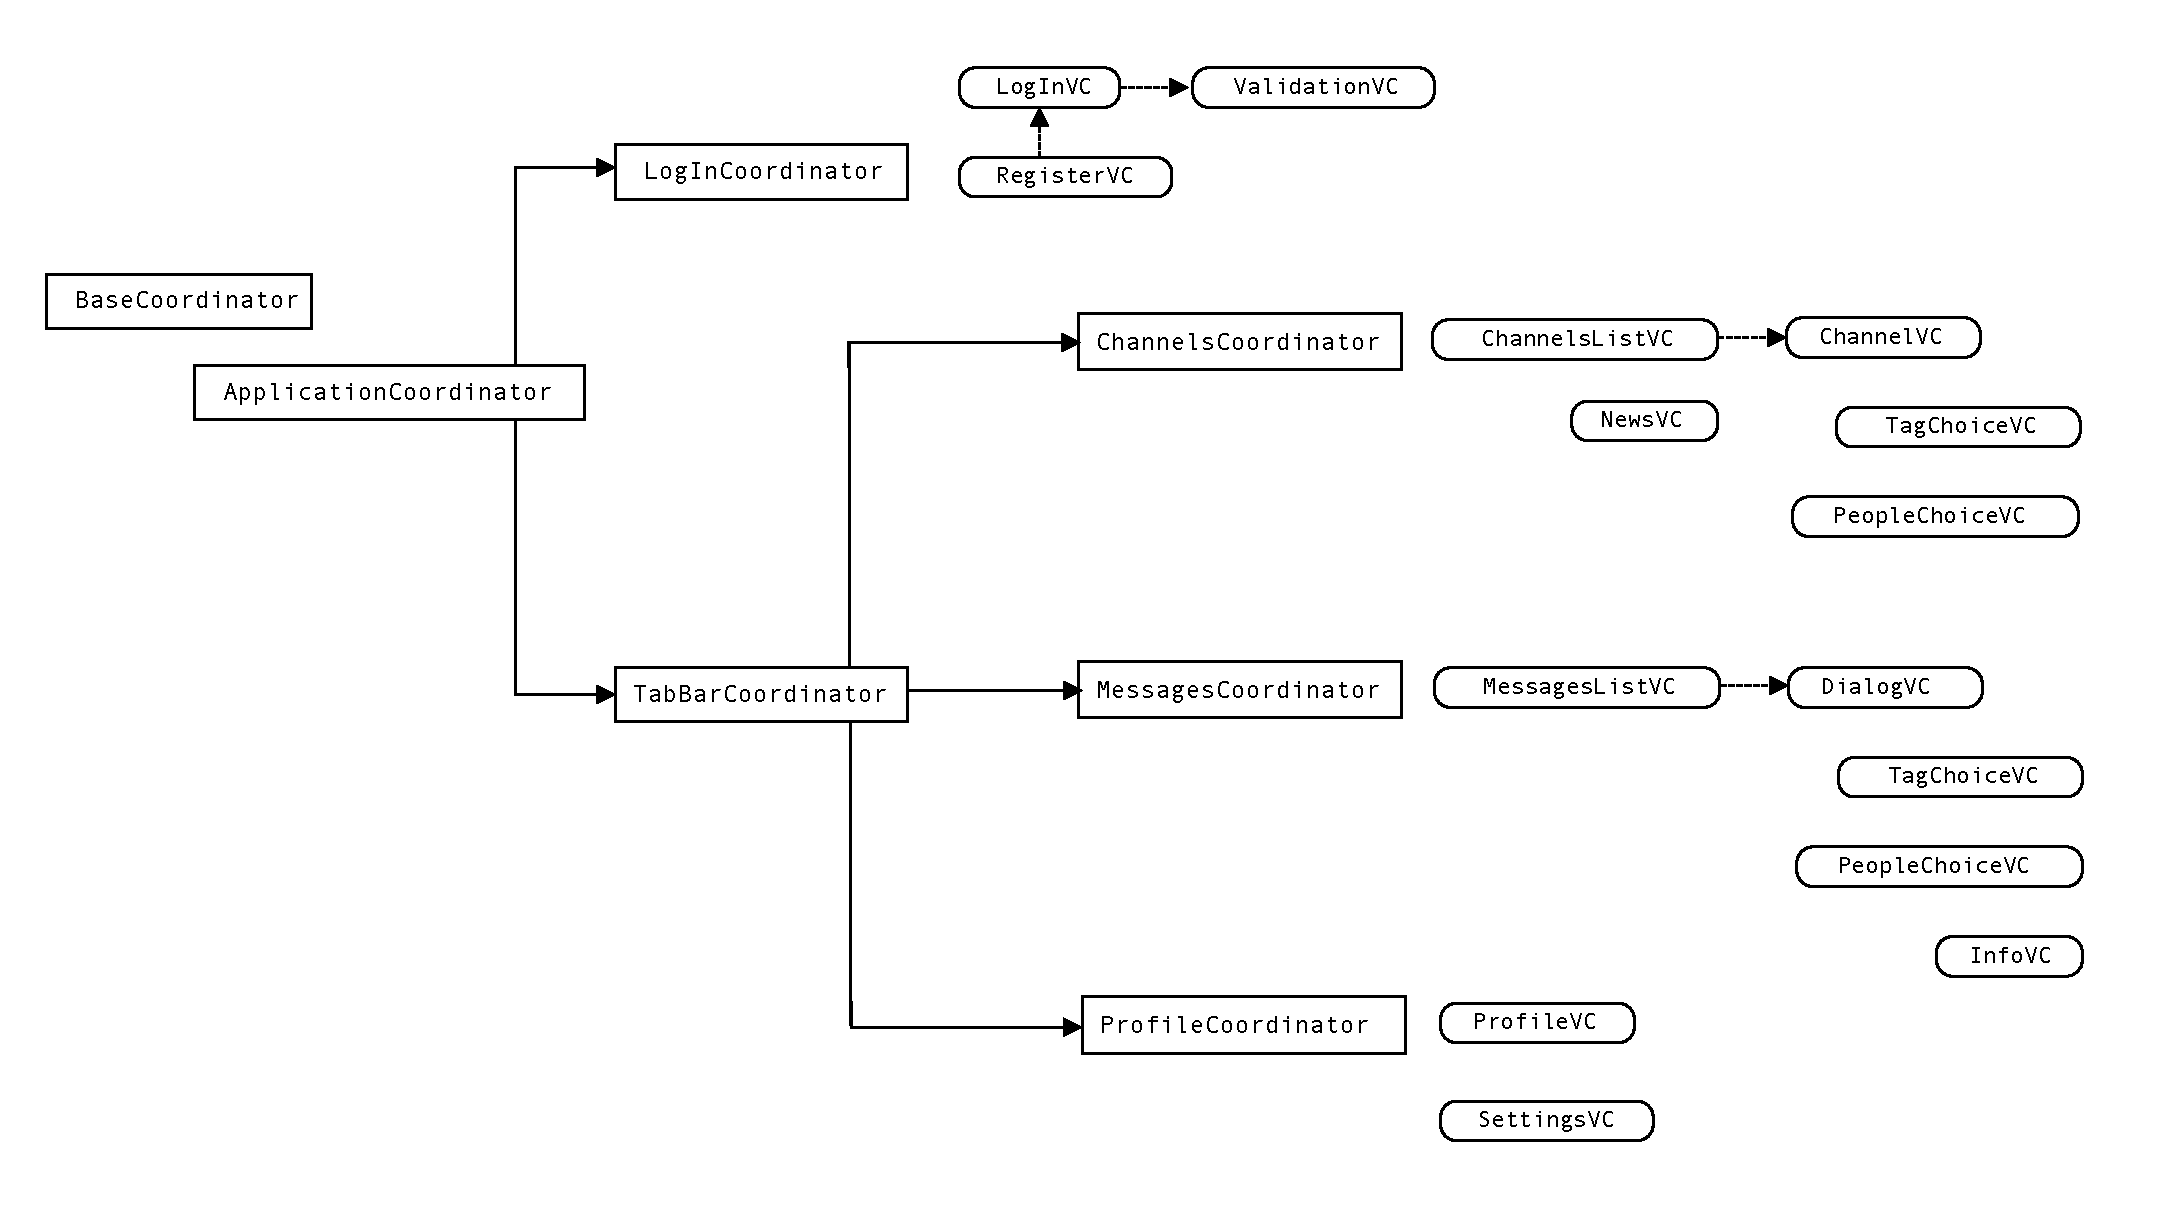
\includegraphics[width = \linewidth]{../includes/illustrations/Flow.pdf}
		\caption{Слои приложения в App Flow}
		\label{pic: Coordinator}
	\end{figure}

	Список слоев управления с описанием их зоны ответственности:
	\begin{enumerate}
		\item AppCoordinator: управление основным Flow программы.\\ Наследуется от \verb|BaseCoordinator|, который в свою очередь правляет зависимостями между координаторами и началом и окончанием работы координаторов.\\ \verb|AppCoordinator| принимает решение, кому передавать работу: схеме авторизации/входа в аккаунт или же начинать работу с авторизованным пользователем в \verb|MainFlow|
		\begin{enumerate}
			\item \verb|LogInCoordinator| отвечает за переключение между авторизацией/регистрацией. В случае успешной авторизации передает работу \verb|TabBarCoordinator|
			\item \verb|TabBarCoodinator| отвечает за \verb|MainFlow| программы. Управляет каналами, сообщениями, профилем до выхода из аккаунта (в этом случае передает работу AppCoodrinator, который в свою очередь делегирует работу \verb|LogInCoordinator|)		
			\begin{enumerate}
				\item \verb|ChannelsCoordinator| координирует работу каналов
				\item \verb|MessagesCoordinator| координирует работу сообщений
				\item \verb|ProfileCoordinator| координирует работу 
			\end{enumerate}
		\end{enumerate}
	\end{enumerate}

	\paragraph{Схема отправки запросов серверу и получения ответа\\}
	Так как приложение <<Социальная сеть для сотрудников НИУ ВШЭ>> является клиент-серверным приложением, то ключевая задача приложения - взаимодействие с сервером \cite{server}: отправка и получение данных. Для корректного отправления и получения данных используется библиотека Alomofire \cite{Alomofire} и возможности стандартной библиотеки iOS SDK (Codable protocol, URLrequest) \cite{SDK}.
	
	Ниже описан класс стандартного запроса \verb|GeneralRequest|. Этот класс позволяет сериализовать в JSON объект типа \verb|GeneralRequest|, который используется для всех запросов постов/сообщений/постов в каналах:
	\code{../includes/code/GeneralRequest.swift}{Структура запроса на сервер}
	
	В классе \verb|Model| содержатся статические методы для отправки конкретных запросов: \verb|POST /posts/forUser|, \verb|POST /posts/last|, \verb|POST /channel/get|,\\ \verb|POST /messages/get/userChat|, \verb|POST /messages/get/groupChat|. Отправка и получение запросов происходит по следующей схеме (ниже приведен пример реализации запроса и возвращения response от сервера):
	
	%\code{includes/code/SimpleRequestExample.swift}
	
	\begin{enumerate}
		\item Создание \verb|URLRequest| с помощью url (iOS SDK)
		\item Сериализация JSON объекта класса \verb|Channels: Codable| (iOS SDK)
		\item Отправка request и получение respose (Alomofire) и валидация полученного \verb|statusCode| от сервера. 
		\item В некоторых случаях происходит десериализация полученного \verb|JSONresponse| с помощью iOS SKD и через \verb|@escaping| замыкание происходит возвращение полученного объекта
	\end{enumerate}
	\paragraph{Схема работы с каналами\\}
	Ниже приведена визуализация управления слоя \verb|ChannelsCoordinator|
	\begin{figure}[h!]
		\centering
		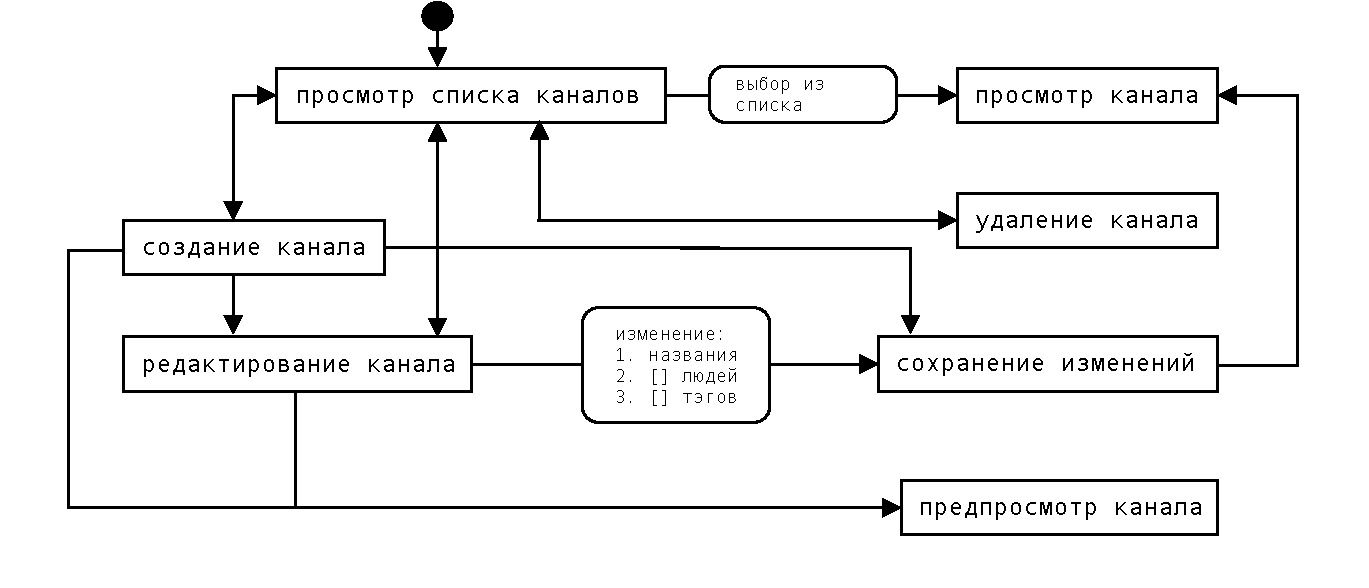
\includegraphics[width = \linewidth]{../includes/illustrations/channelsFlow.pdf}
		\caption{Диаграмма состояний}
		\label{pic: channel}
	\end{figure}

	Процесс работы клиента с каналами выглядит следующим образом (см. рис \ref{pic: channel}):
	\begin{itemize}
		\item Запрос данных на сервер для отображения списка каналов
		\begin{itemize}
			\item При успешном запросе пользователь видет список каналов
			\item При ошибке запроса (\verb|statusCode != 200|) - демонстрируется пустая таблица
		\end{itemize}
		\item При редактировании или создании канала происходит вызов методов updateChannel или createChannel
		\begin{itemize}
			\item При успешном запросе пользователь видет только что созданный/измененный канал в списке каналов
			\item При ошибке запроса (\verb|statusCode != 200|) изменения к выбранному каналу не применяются
		\end{itemize}
		Запрос на сервер осуществляется при выходе из режима редактирования канала с последующим обновлением списка каналов
		\item При выборе режима просмотра содержимого канала отправляется запрос на сервер
		\begin{itemize}
			\item При успешном запросе пользователь видет ленту, отвечающую множестам подписок на канал
			\item При ошибке запроса (\verb|statusCode != 200|) пользователь видит пустую ленту канала
		\end{itemize}
	\end{itemize}
\clearpage
\paragraph{Схема работы с сообщениями\\}
Ниже приведена визуализация cлоя, отвечающего за работу с сообщениями:
\begin{figure}[h]
	\centering
	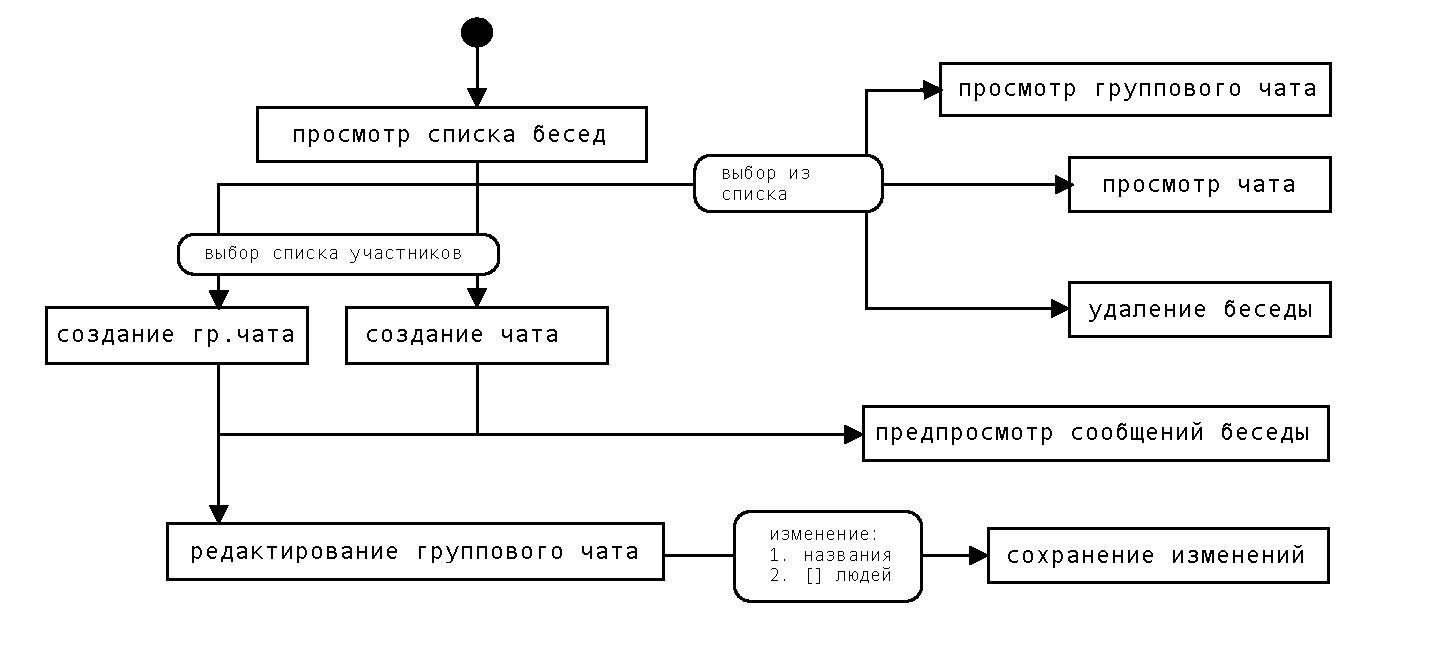
\includegraphics[width = 0.8\linewidth]{../includes/illustrations/Messages.pdf}
	\caption{Диаграмма состояний}
	\label{pic: messages}
\end{figure}

Процесс работы клиента с сообщениями (см. рис \ref{pic: messages}, \ref{pic: pmessages}) выглядит следующим образом:
\begin{itemize}
	\item Запрос данных на сервер для отображения списка диалогов
	\begin{itemize}
		\item При успешном запросе пользователь видет список чатов и бесед
	\end{itemize}
	\item При просмотре сообщений клиент имеет возможность пролистывать сообщения в обратном хронологическом порядке, для этого серверу отправляются запросы в формате <<с какого сообщения>>, <<сколько>>, <<какое направление>>
	\item При выходе из режима редактирования беседы происходит update с отправлением новой информации о чате на сервер
\end{itemize}
\begin{figure}[h!]
	\centering
	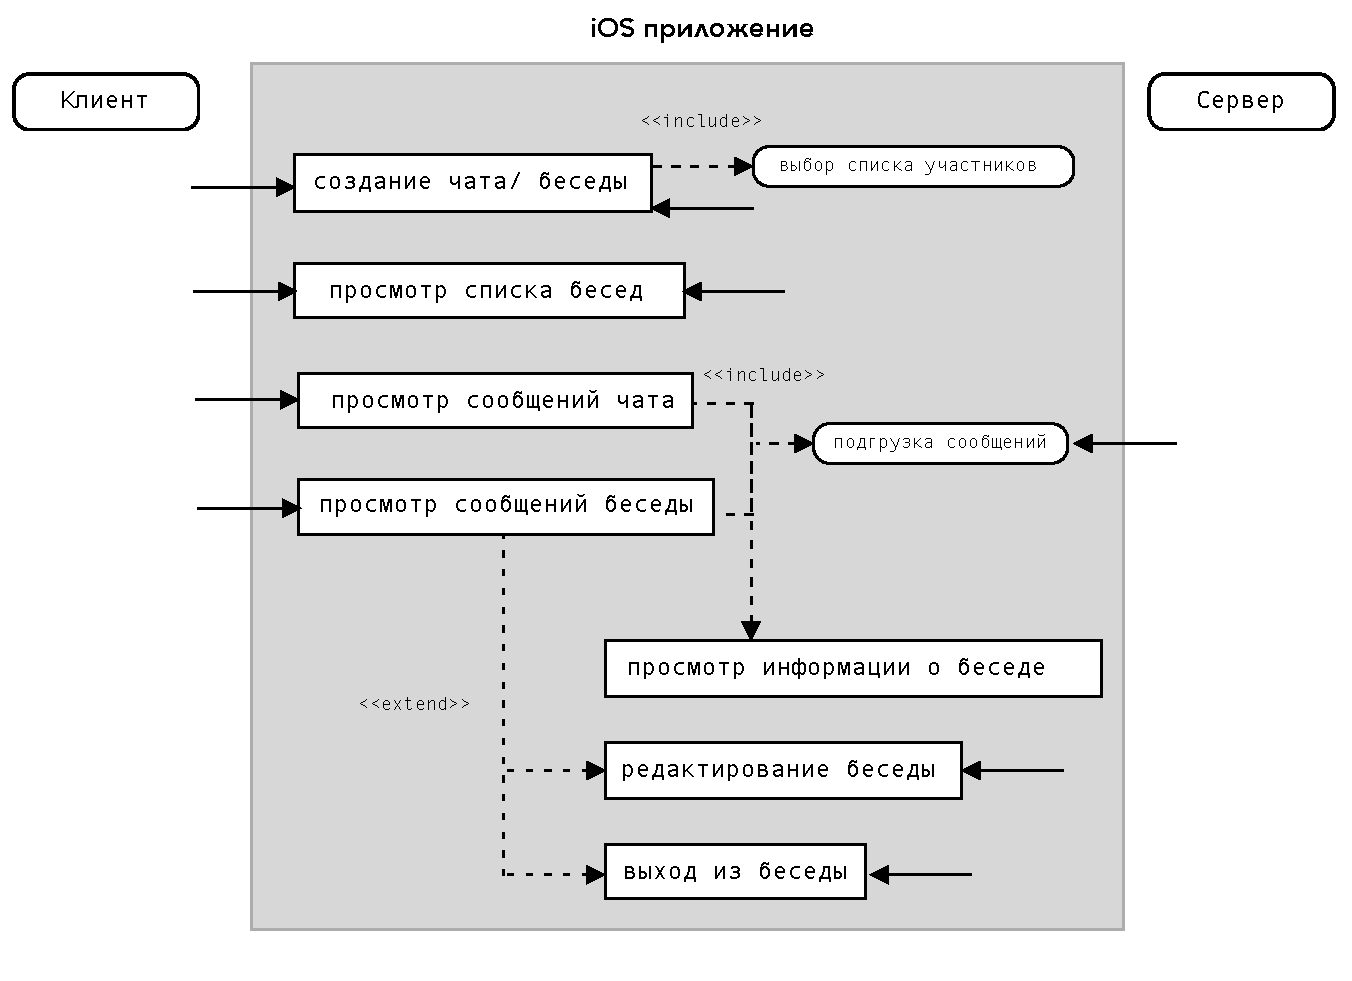
\includegraphics[width = 0.7\linewidth]{../includes/illustrations/PMessages.pdf}
	\caption{Диаграмма прецедентов}
	\label{pic: pmessages}
\end{figure}
\clearpage	
	
	\paragraph{Схема авторизации и регистрации клиента\\}
	При входе в аккаунт пользователю предлагается ввести свою почту (см. рис \ref{pic: auth}, \ref{pic: authP}):
	\begin{enumerate}
		\item Процесс входа уже зарегистрированного пользователя:
		\begin{enumerate}
			\item Ввод email -- происходит отправка запрос на сервер для валидации данных, получение ответа от сервера и cookies для header запросов
			\item При успешной валидации почты на сервере, происходит получение письма на введенную почту с кодом подтверждения 
			\item Клиент вводит полученный код в специальное поле -- при успешной валидации кода полученные cookies становятся активными и клиент успешно входит в приложение
		\end{enumerate}
	\item Процесс регистрации:
		\begin{enumerate}
			\item Ввод email -- происходит отправка запрос на сервер для валидации данных
			\item При успешной валидации почты на сервере, происходит получение письма на введенную почту с кодом подтверждения 
			\item Клиент вводит полученный код в специальное поле -- при успешной валидации кода клиент получает cookies для header запросов
			\item Открывается окно с регистрацией: пользователю необходимо заполнить обязательные поля (см. раздел требований \ref{req: auth})
			\item После заполнения пользователь подтверждает создание учетной записи, объект с заполненныи данными пользователя отправляется на сервер, cookies становятся активными и клиент успешно входит в приложение
		\end{enumerate}
	\end{enumerate}
	\begin{figure}[h!]
		\centering
		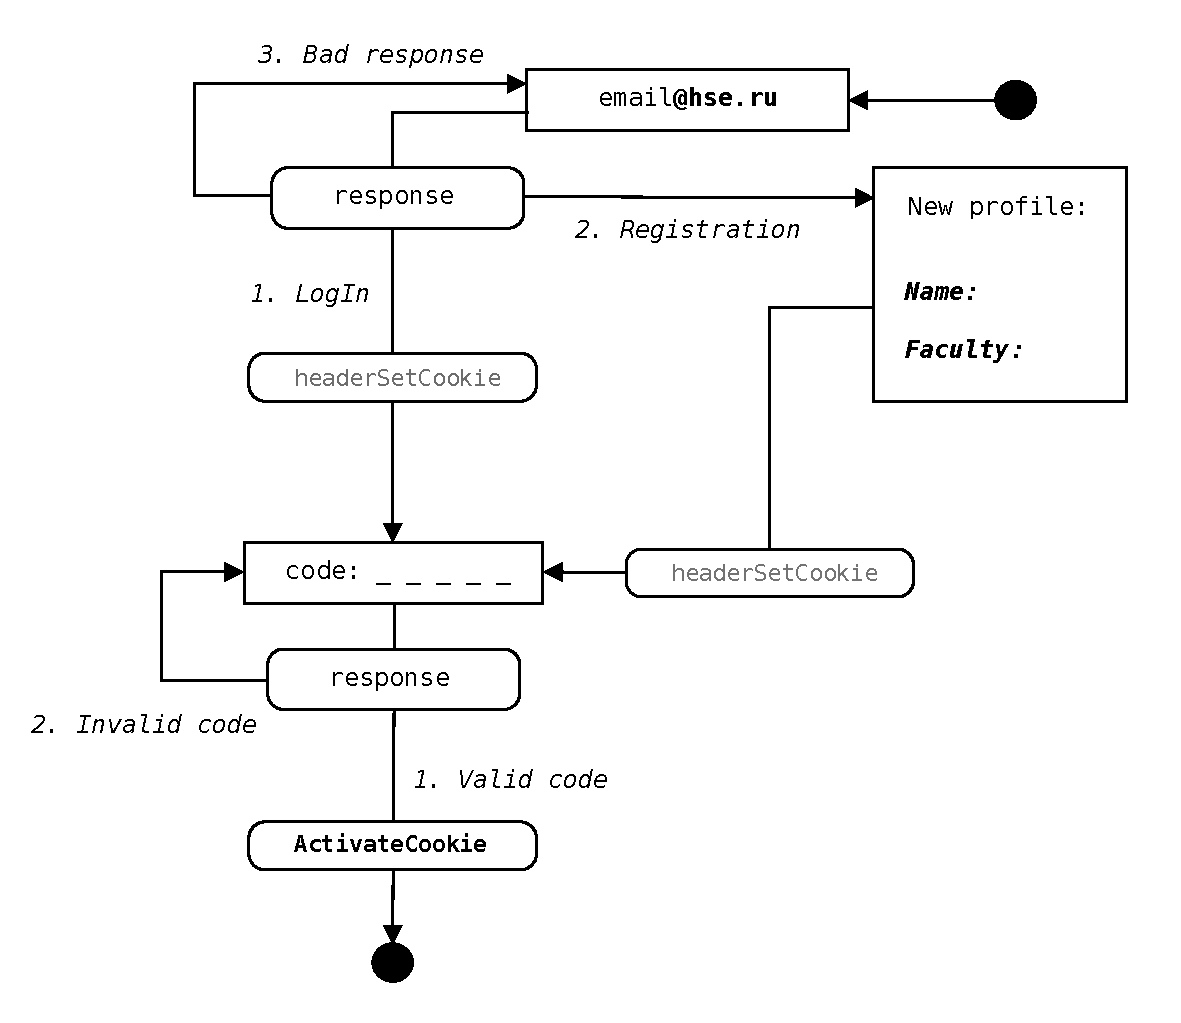
\includegraphics[width = 0.7\linewidth]{../includes/illustrations/Auth.pdf}
		\caption{Диаграмма состояний}
		\label{pic: auth}
	\end{figure}

	\begin{figure}[h!]
		\centering
		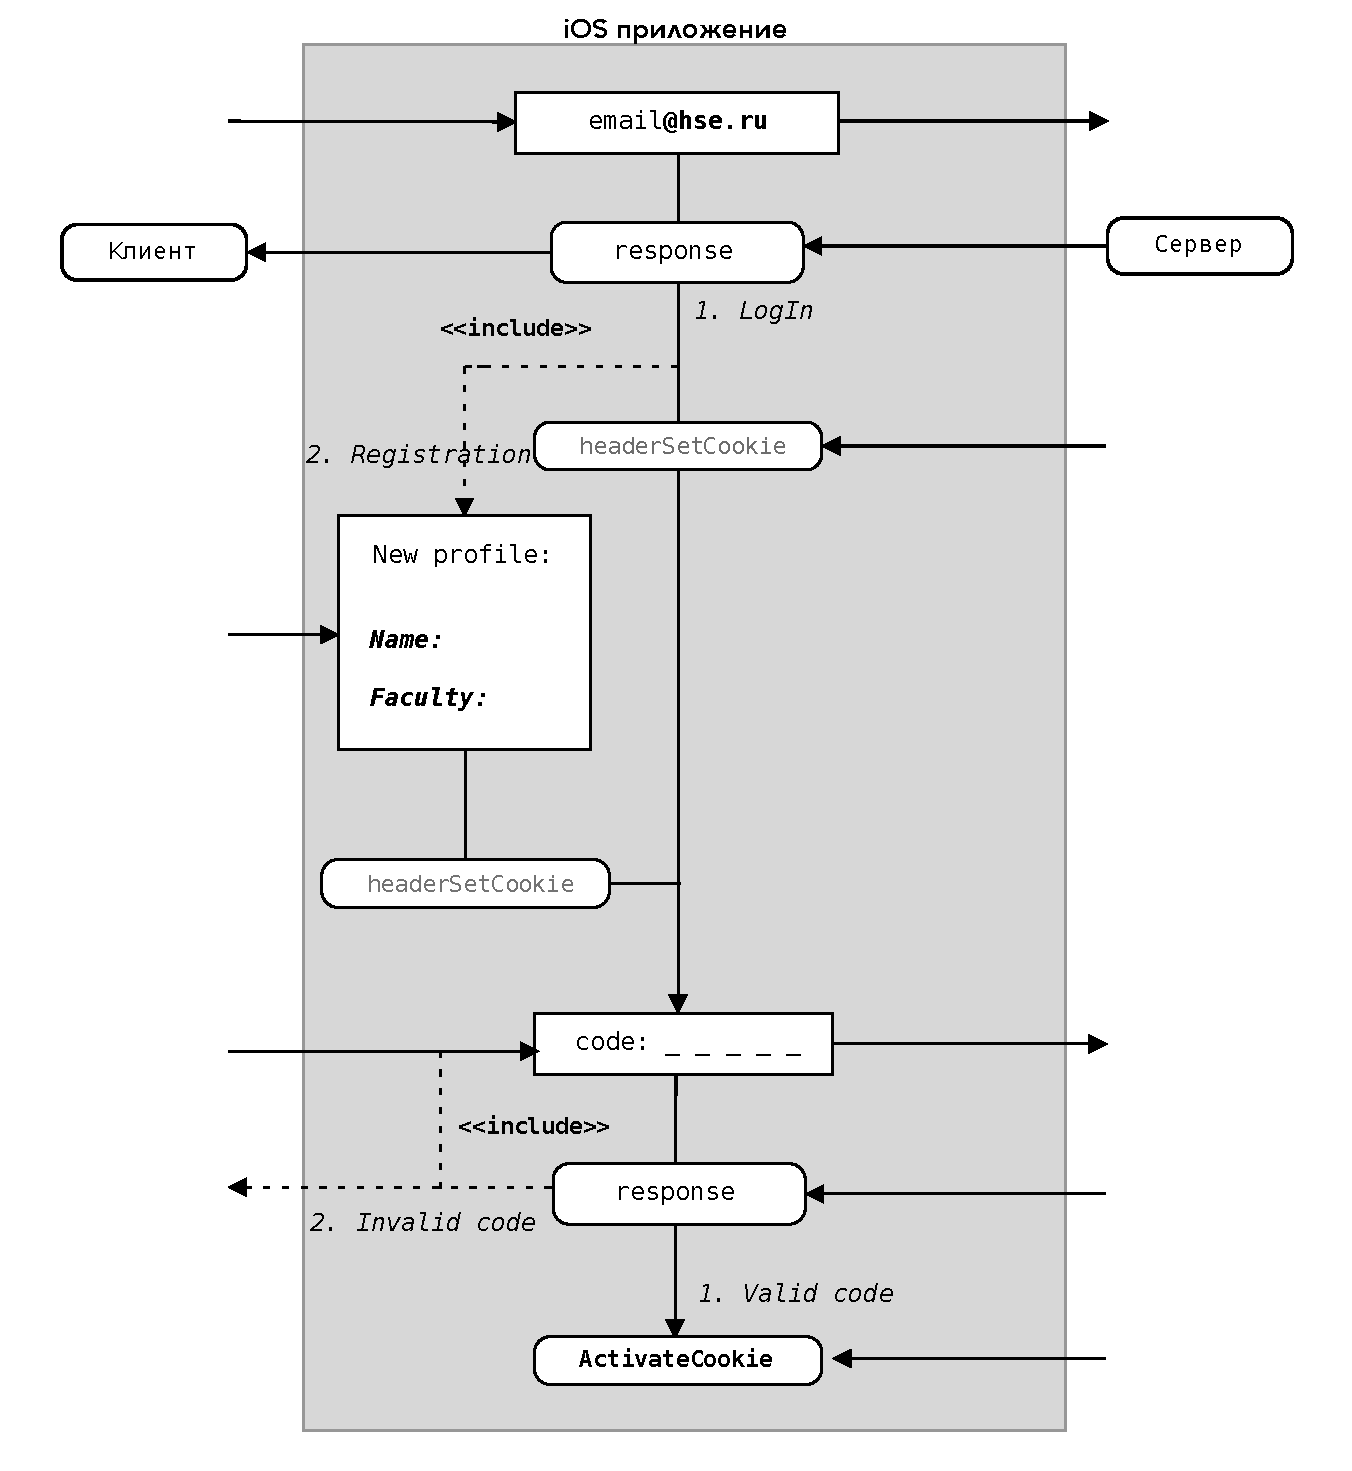
\includegraphics[width = \linewidth]{../includes/illustrations/AuthP.pdf}
		\caption{Диаграмма прецедентов}
		\label{pic: authP}
	\end{figure}
	\clearpage	
	\subsubsection{Возможные взаимодействия программы с другими программами}
	
	Приложение <<Социальная сеть для сотрудников НИУ ВШЭ>> разработана с использованием сторонних библиотек: 
	\begin{itemize}
		\item github <<robb/Cartography>>: расстановка ограничений верстки в коде
		\item github <<ivanbruel/MarkdownKit>>: отображение markdown текста в постах
		\item github <<roberthein/TinyConstraints>>: расстановка ограничений верстки в коде
		\item github <<macteo/Marklight>>: поддержка синтаксической подсветки markdown
		\item github <<Alamofire/Alamofire>> <<5.0.0-beta.2>>: для отправки запросов и получения ответов от сервера
		\item github <<ZaidSA/TaggerKit>> (forked from nekonora/TaggerKit): создание хэштегов, поиск и автодополнение
		\item github <<ReactiveCocoa/ReactiveCocoa>>: валидация почты 
	\end{itemize}
	\subsection{Описание и обоснование выбора метода организации входных и выходных данных}
	
	\subsubsection{Описание метода организации входных и выходных данных}
	
	\renewcommand{\labelenumi}{\textbf{FR-\arabic{enumi}}.}

\renewcommand{\labelenumii}{\textbf{FR-\arabic{enumi}.\arabic{enumii}}.}

\renewcommand{\labelenumiii}{\arabic{enumiii}.}
\begin{enumerate}
	\setcounter{enumi}{6}
	\item \textbf{Входные данные\\}
	Одна из основных задач приложения -- создать площадку для коммуникации и обмена информацией между сотрудниками университета.
	 \begin{enumerate}
		\item При регистрации или входе в аккаунт в качестве входных данных программа будет принимать email только с доменом @hse.ru. (см ~\ref{FR-1.2})
		\item При общении, создании постов у пользователей должна быть возможность обмениваться текстовой информацией. 
	\end{enumerate}
\end{enumerate}
\renewcommand{\labelenumi}{\arabic{enumi}.}

\renewcommand{\labelenumii}{\arabic{enumii}.}

\renewcommand{\labelenumiii}{\arabic{enumiii}.}

	
	\renewcommand{\labelenumi}{\textbf{FR-\arabic{enumi}}.}

\renewcommand{\labelenumii}{\textbf{FR-\arabic{enumi}.\arabic{enumii}}.}

\renewcommand{\labelenumiii}{\arabic{enumiii}.}
\begin{enumerate}
	\setcounter{enumi}{7}
	\item \textbf{Выходные данные}
	\begin{enumerate}
		\item Выходные данные должны быть представлены посредством пользовательского интерфейса в качестве информации, полученной через указанные API методы от сервера. 
		\item Все данные, собранные в процессе работы программы, загружаются на сервер во время работы программы и при ее завершении. 
	\end{enumerate}
\end{enumerate}
\renewcommand{\labelenumi}{\arabic{enumi}.}

\renewcommand{\labelenumii}{\arabic{enumii}.}

\renewcommand{\labelenumiii}{\arabic{enumiii}.}

	\subsubsection{Обоснование выбора метода организации входных и выходных данных}
	
	Выбор входных и выходных данных обусловлен установленным функционалом программы.
	
	
	\subsection{Описание и обоснование выбора состава технических и программных средств}
	
	
	\subsubsection{Состав технических и программных средств}
	При разработке программного продукта использовались следующие технические и программные средства:
	\begin{itemize}
		\item Язык разработки: Swift 5.0
		\item Среда разработки: Xcode Version 10.2.1
		\item Dependency manager: Carthage
		\item iPhone 7 версии 12.2
		\item Библиотеки, использованные при разрабоке: github <<robb/Cartography>>, github <<ReactiveCocoa/ReactiveCocoa>>, github <<ZaidSA/TaggerKit>> \\ (forked from nekonora/TaggerKit), github <<ivanbruel/MarkdownKit>>, \\ github <<roberthein/TinyConstraints>>, github <<macteo/Marklight>>,\\ github <<Alamofire/Alamofire>>
	\end{itemize}
	\subsubsection{Обоснование выбора состава технических и программных средств}
	\paragraph{Язык программирования\\}
	Компания Apple поддерживает два языка программирования для iOS разработки: Objective-C и Swift. 
	
	Для разработки был выбран язык Swift 4.2, так как он более легкий в изучении, прост и приятен в синтаксисе, level of performance выше более чем в 1.5 раза чем у других языков, на которых можно разрабатывать под iOS платформу \cite{whySwift}. В процессе работы проект мигрировал на новую версию Swift 5.0 (первая ABI стабильная версия).
	\paragraph{Среда разработки\\}
	Так как изначально было принято решение разрабатывать нативное приложение на языке программирования Swift, то такие среды разработки как Xamarin не рассматривались. Xcode -- бесплатная (в отличие от AppCode) и удобная среда разработки  нативных приложений на iOS, разработанная компанией Apple.
	
	\paragraph{Шаблон проектирования\\}
	
	Был выбран шаблон проектирования MVC: он используется в iOS SDK и рекомендован производитем платформы. Другие основные паттерны, использованные при разработке: delegation, Coodinator pattern.
	\paragraph{Библиотеки}
	
	\begin{description}
		\item [Alomofire] библиотека HTTP запросов для Swift. Эта библиотека используется для выполнения всех запросов на сервер \cite{server} и получения данных. Удобное API для error handling, responce handling.
		\item [TinyConstraints/Cartography] - обе библиотеки использовались для расставлений размеров и накладываний ограничений на внешний вид элементов \verb|self.view| в коде. Xcode поддерживает \verb|autolayout| с помощью технологии выставления constraints в \verb|storyboard|, но этот способ не подходит для сложных лэйаутов/анимаций. Обе библиотеки имеют документацию, содержащую информацию о том, как реализовывать расставление, анимацию constraints непосредственно в коде приложения. Несколько viewControllers были созданы полностью с помощью кода (не использовался \verb|storyboard|), эти библиотеки помогли создать \verb|layout| без xml поддержки. iOS SDK также поддерживает возможность расставлять ограничения в коде, но стандартная библиотека предоставляет неудобный API для этого. В частности Cartography позволяет объединять constraints  в группы, эта возможность позволяет в динамике работать со взаимосвязанными объектами и их размерами. Библиотека TinyConstraints - синтаксический сахар, заменяющий длинные строчки кода из стандартной библиотеки на маленький и емкий кусок кода.
		\item [MarkdownLight/Marklight/TaggerKit] - библиотеки использовались для парсинга маркдауна/подстветки синтаксиса и представления выбора хэштегов в приложении. Все три библиотеки не подразумевают сложного API, не требуют дополнительных знаний
	\end{description}
	
						\newpage
	\section{Технико-экономические показатели}
	\subsection{Предполагаемая потребность}
	Программа будет использоваться сотрудниками НИУ ВШЭ для коммуникации между научными сотрудниками, преподавателями, сотрудниками с разных факультетов.
	
	% ЭКСПЛУАТАЦИОННОЕ НАЗНАЧЕНИЕ

Программа будет использоваться как средство общения и огранизации работы над совместными научными проектами между сотрудниками с одного или разных направлений/ факультетов/ кампусов. 


Таким образом, программный продукт позволит решить проблему коммуникации между факультетами, кампусами НИУ ВШЭ и даст возможность наладить взаимодействие между преподавателями университета, будет способствовать развитию научной деятельности между разными факультетами и кампусами.
	\subsection{Экономические преимущества по сравнению с отечественными и зарубежными аналогами}
	% Ориентировочная экономическая эффективность
% 
% dyurednikina
% version 1.0
% date 11.11.2018

В данной таблице приведен список прямых и косвенных конкурентов социальной сети.
\begin{longtable}{|r|c|l|} 
\caption{Виды конкурентов} \label{t:competetors0}\\
	  \hline
	\textbf{Название} & \textbf{Описание} & \textbf{Вид} \\ \hline
\textbf{Вк} &Социальная сеть& Прямой \\ \hline
\textbf{Твиттер} &Социальная сеть& Прямой \\ \hline
\textbf{Телеграмм} &Социальная сеть& Прямой \\ \hline
\textbf{Ватсап} &Мессенджер& Прямой \\ \hline
\textbf{Фейсбук} &Социальная сеть& Прямой \\ \hline
\textbf{Лмс} &Система организации обучения& Прямой \\ \hline
\textbf{Официальный сайт} &Информационный портал& Прямой \\ \hline
\textbf{Слак} &Социальная сеть& Прямой \\ \hline
\textbf{Вайбер} &Мессенджер& Прямой \\ \hline
\textbf{LinkedIn} &Социальная сеть& Прямой \\ \hline
\textbf{Одноклассники} &Социальная сеть& Прямой \\ \hline
\textbf{Мероприятия} &Конференции& Косвенный \\ \hline
\textbf{Instagram} &Социальная сеть& Прямой \\ \hline
\textbf{Почта} &Способ рассылки сообщений& Косвенный \\ \hline
\textbf{Brainly} &Социальная сеть& Прямой \\ \hline
\textbf{Skype} &Социальная сеть& Прямой \\ \hline
\textbf{ResearcherGate} &Социальная сеть& Прямой \\ \hline
\textbf{Mendeley} &Социальная сеть& Прямой \\ \hline
\textbf{ieee-collabaratec} &Социальная сеть& Прямой \\ \hline
\textbf{Authorea} &Социальная сеть& Прямой \\ \hline
\textbf{Edmodo} &Социальная сеть& Прямой \\ \hline
\end{longtable}


Большинство аналогов не ориентированы на научную деятельность. 
Прямые конкуренты (например, LMS) не удовлетворяют всем перечисленным критериям (не имеют приложения на мобильные устройства, нет возможности предпросмотра кода, бесперебойность работы). 


Таким образом, приложение <<Социальная сеть для сотрудников НИУ ВШЭ>> будет пользоваться спросом среди сотрудников НИУ ВШЭ из-за его узкой направленности (приложение могут использовать только сотрудники университета), ориентации на развитие научной деятельности, наличии приложения и бесперебойной работы социальной сети.


Ниже приведена таблица с детальным анализом конкурентов социальной сети. При подсчете финальной оценки кажого конкурента большим приоритетом в формуле обладали показатели критериев <<Ориентированность на профессионаоьную и исследовательскую деятельность>>, <<Бесперебойность работы>> и <<Категоризация информации>>. Именно эти критерии наиболее релевантны для будущих пользователей разрабатываемого приложения.

\renewcommand{\labelenumi}{\textbf{\Alph{enumi}}.}

\renewcommand{\labelenumii}{\textbf{\alph{enumi}\arabic{enumii}}}

Для вычисления финальной оценки был применен следующий алгоритм: 
критерии оценки были разбиты на следующие кластеры исходя из смысла, для каждой категории был задан вес(от 0 до 10, где 10 -- самое важное) исходя из общих рассуждений о важности: 
\begin{enumerate}
	
	\item Наличие бесед -- 10
	\item Поиск по категориям -- 9
	\item Категоризация информации -- 9
	\item Автоматический выбор релевантной информации -- 9
	\item Ориентированность на профессиональную деятельность -- 8
	\item Подгрузка информации из релевантных источников -- 3
	\item Ориентированность на мобильные устройства -- 9
	\item Наличие десктопного приложения -- 9
	\item Наличие web-версии -- 9
	\item Код -- 8
	\item Мультиплатформенность -- 9
	\item Мультимедиа -- 6
	\item Разделение сообщения/объявления/профиль -- 9
	\item Бесперебойность работы -- 8
\end{enumerate}
Итоговый коэффициент для каждой оценки рассчитывался, как 
\begin{equation}
\frac{n}{\sum_{i = 1}^7 n} \label{eq}
\end{equation} 

%где n - вес конкретной оценки \eqref{eq}\\
Финальная оценка рассчитывалась по следующей формуле:\\

\code{../includes/code/coeff.py}{Функция, рассчитывающая финальную оценку}


\newpage
%\newgeometry{left=0cm, top=0cm,right=0cm,bottom=0cm}
{

\footnotesize

\begin{longtable}{| >{\raggedright\arraybackslash}p{2.7cm}| >{\centering\arraybackslash}p{0.2cm}| p{0.2cm}| p{0.2cm}| p{0.2cm}| p{0.2cm}| p{0.2cm}| p{0.2cm}| p{0.2cm}| p{0.2cm}| p{0.2cm}| p{0.2cm}| p{0.2cm}| p{0.2cm}| p{0.2cm}| p{0.2cm}| p{0.2cm}| p{0.2cm}| p{0.2cm}| p{0.2cm}| p{0.2cm}|}
	\caption{Детальный анализ конкурентов} \label{t:an} \\
\hline
& \rotatebox{-90}{\textbf{Вк}} & \rotatebox{-90}{\textbf{Твиттер}} & \rotatebox{-90}{\textbf{Телеграмм}} & \rotatebox{-90}{\textbf{Ватсап}} & \rotatebox{-90}
{\textbf{Фейсбук}} & \rotatebox{-90}{\textbf{Лмс}} & \rotatebox{-90}{\textbf{Официальный сайт\ }} & \rotatebox{-90}{\textbf{Слак}} & \rotatebox{-90}{\textbf{Вайбер}} & \rotatebox{-90}{\textbf{Mendeley}} & \rotatebox{-90}{\textbf{Одноклассники}} & \rotatebox{-90}{\textbf{Мероприятия}} & \rotatebox{-90}{\textbf{Instagram}} & \rotatebox{-90}{\textbf{Почта}} & \rotatebox{-90}{\textbf{Brainly}} & \rotatebox{-90}{\textbf{Skype}} &\rotatebox{-90}{\textbf{ResearcherGate}} &\rotatebox{-90}{\textbf{ieee-collabratec}} & \rotatebox{-90}{\textbf{Authorea}}& \rotatebox{-90}{\textbf{Edmodo}}\\ \hline


 \endfirsthead

 \caption*{Продолжение Таблицы \ref{t:an}}  \\

 \hline
 \endhead
 \hline

 \caption*{ Продолжение на след. странице} \
 \endfoot
 \endlastfoot
\textbf{Наличие бесед} & 7 & 3 & 10 & 8 & 8 & 0 & 0 & 10 & 7 & 2 & 7 & 10 & 4 & 0 & 0 & 6 & 0& 6& 0& 8 \\ \hline
\textbf{Поиск по категориям} & 7 & 8 & 4 & 2 & 7 & 0 & 4 & 9 & 0 & 5 & 4 & 3 & 7 & 5 & 9 & 0 & 9& 8& 8& 8 \\ \hline
\textbf{Категоризация информации} & 4 & 5 & 2 & 2 & 4 & 7 & 7 & 8 & 0 & 6 & 4 & 8 & 6 & 5 & 8 & 0 & 9& 7& 8& 7 \\ \hline
\textbf{Ориентирован- ность на профессиональную исследовательскую деятельность} & 2 & 2 & 2 & 2 & 2 & 10 & 10 & 9 & 0 & 10 & 2 & 10 & 1 & 8 & 10 & 4 & 10 & 10& 10& 6\\ \hline
\textbf{Подгрузка информации из других релевантных источников} & 3 & 3 & 3 & 0 & 5 & 0 & 0 & 10 & 0 & 8 & 0 & 0 & 0 & 0 & 0 & 0 & 0& 5& 5 & 8\\ \hline
\textbf{Автомати- ческий выбор релевантной информации} & 6 & 6 & 0 & 0 & 6 & 0 & 0 & 0 & 0 & 7 & 0 & 0 & 6 & 0 & 0 & 0 & 8 & 7& 6& 8\\ \hline
\textbf{Ориентирован- ность на мобильные устройства} & 9 & 7 & 9 & 9 & 8 & 0 & 5 & 8 & 6 & 4 & 5 & 0 & 8 & 9 & 7 & 7 & 4 & 4& 5& 10\\ \hline
\textbf{Наличие десктопного приложения} & 6 & 0 & 8 & 3 & 0 & 0 & 0 & 8 & 3 & 8 & 0 & 0 & 2 & 9 & 0 & 7 & 0 & 0 & 0& 0\\ \hline
\textbf{Наличие web-версии} & 10 & 7 & 8 & 3 & 10 & 6 & 10 & 8 & 4 & 6 & 10 & 4 & 2 & 9 & 10 & 5 & 7& 3& 8& 9 \\ \hline

\textbf{Мультимедиа} & 9 & 6 & 7 & 6 & 8 & 2 & 2 & 6 & 5 & 5 & 8 & 4 & 7 & 6 & 4 & 5 & 7& 9 & 9& 8\\ \hline
\textbf{Код} & 0 & 0 & 4 & 0 & 0 & 0 & 0 & 9 & 0 & 0 & 0 & 0 & 0 & 0 & 3 & 0 & 9 & 10& 9& 6\\ \hline
\textbf{Разделение сообщения/ объявления/ профиль} & 8 & 7 & 4 & 4 & 8 & 7 & 3 & 5 & 4 & 4 & 7 & 7 & 4 & 0 & 2 & 5 & 8 & 7& 6& 10\\ \hline
\textbf{Бесперебой- ность работы} & 9 & 8 & 5 & 10 & 10 & 6 & 10 & 10 & 10 & 9 & 10 & 7 & 10 & 10 & 10 & 8 & 10 & 2& 8& 10\\ \hline
\textbf{Финальная оценка} & \textbf{\scriptsize \kern-0.3em 6.7} & \textbf{\scriptsize \kern-0.3em 5.1} & \textbf{\scriptsize \kern-0.3em 5.9} & \textbf{\scriptsize \kern-0.3em 4.7} & \textbf{\scriptsize \kern-0.3em 6.9} &\textbf{\scriptsize \kern-0.3em 2.7} &\textbf{\scriptsize \kern-0.3em 4.2} & \textbf{\scriptsize \kern-0.3em 8.5} & \textbf{\scriptsize \kern-0.3em 4.1} & \textbf{\scriptsize \kern-0.3em 5.7} & \textbf{\scriptsize \kern-0.3em 5.5} &\textbf{\scriptsize \kern-0.3em 5.2} &\textbf{\scriptsize \kern-0.3em 4.5} & \textbf{\scriptsize \kern-0.3em 4.9} & \textbf{\scriptsize \kern-0.3em 5.1} & \textbf{\scriptsize \kern-0.3em 4.5} & \textbf{\scriptsize \kern-0.3em 5.9} & \textbf{\scriptsize \kern-0.3em 5.9} & \textbf{\scriptsize \kern-0.3em 6}& \textbf{\scriptsize \kern-0.3em 8.2}\\ \hline
\end{longtable}
}
\newpage
%\restoregeometry


\renewcommand{\labelenumi}{\arabic{enumi}.}

\renewcommand{\labelenumii}{\arabic{enumii}.}

\renewcommand{\labelenumiii}{\arabic{enumiii}.}




\newpage
\patchcmd{\thebibliography}{\section*{\refname}}{}{}{}
\addition{Список литературы}
% приложения нумеруются отдельно и надо выровнять по правому краю
%\section{Источники, использованные при разработке}
%\renewcommand{\refname}{Список источников}
%\addcontentsline{toc}{section}{\refname}
\begin{thebibliography}{7}
	\bibitem{iOS} The Swift Programming Language Documentation [Электронный ресурс] URL: \url{https://swift.org/documentation/#the-swift-programming-language} (Дата обращения: 16.05.2019, режим доступа: свободный)
	\bibitem{documentation}Единая система программной документации – М.: ИПК, Издательство стандартов, 2000, 125 стр.
	\bibitem{server} GitHub repository ilyakoo0/denis [Электронный ресурс] URL: \url{https://github.com/ilyakooo0/denis} (Дата обращения: 16.05.2019, режим доступа: свободный)
	
	\bibitem{Alomofire} GitHub repository Alomofire/Alomofire [Электронный ресурс] URL: \url{https://github.com/Alamofire/Alamofire} (Дата обращения: 16.05.2019, режим доступа: свободный)
	\bibitem{SDK} Swift Standard Library [Электронный ресурс] URL: \url{https://developer.apple.com/documentation/swift/swift_standard_library} (Дата обращения: 16.05.2019, режим доступа: свободный)
	
	\bibitem{lms} 
	LMS [Электронный ресурс] URL: 
	\url{https://lms.hse.ru} (Дата обращения: 16.05.2019, режим доступа: свободный)
	
	\bibitem{whySwift} 
	Aticle <<9 Reasons to Choose Swift for iOS App Development>> [Электронный ресурс] URL: 
	\url{https://www.upwork.com/hiring/for-clients/9-reasons-to-choose-swift-for-ios-app-development/} (Дата обращения: 16.05.2019, режим доступа: свободный)
\end{thebibliography}

\newpage

\addition{Используемые понятия и определения}
\begin{description}
		\item[Социальная сеть] -- это интернет-площадка, сайт, который позволяет зарегистрированным на нем пользователям размещать информацию о себе и коммуницировать между собой, устанавливая социальные связи
		\item[Хэштег] -- ключевое слово или несколько слов сообщения, тег (пометка), используемый в микроблогах и социальных сетях, облегчающий поиск сообщений по теме или содержанию и начинающийся со знака решётки \label{term: hash}
		\item[Пост] -- информационный блок, размещённый пользователем в социальной сети на своей странице и содержащий набор хэштегов, по которым его можно найти \label{term: post}
		\item[Канал] -- сохраненные ранее созданные фильтры новостей (набор хэштегов) по всем публичным постам \label{term: channel}
		\item [Беседа] -- чат для пользователей, в котором одновременно могут присутствовать от 3 до 50 участников \label{term: chat}
		\item [Проект]  -- раздел, в котором сотрудники с любых факультетов по приглашению смогут вместе работать над каким-либо научным исследованием. Проект состоит из timeline (лента с новостями для всех участников проекта) и набором чатов и бесед (с разным количеством участников в каждой) \label{term: project}
		\item [Preview канала]  -- предпросмотр ленты канала с ограничениями на просмотр полной версии поста в ленте, переходом на страницы авторов, нажатия на хэштеги \label{term: preview}
		\item [Preview поста]  -- ограниченный контент (содержание) поста в ленте \label{term: previewPost}
		\item [Model-View-Controller] MVC схема разделения данных приложения, пользовательского интерфейса и управляющей логики на три отдельных компонента: модель, представление и контроллер — таким образом, что модификация каждого компонента может осуществляться независимо
		\item [Xcode] интегрированная среда разработки (IDE) программного обеспечения для платформ macOS, iOS, watchOS и tvOS, разработанная корпорацией Apple
		\item [Dependency manager] программный модуль, который координируют интеграцию внешних библиотек или пакетов в стек приложения
		\item [Constraints] ограничения на размеры и положения объектов на view,  необходимые для правильного определения размеров и позиций контейнеров
		\item [Storyboard] удобный механизм разработки интерфейса программы
	\end{description} %термины и определения

\addition{Статус требований}
\begin{longtable}{|p{0.2\linewidth}|p{0.5\linewidth}|} 
	\caption{Статус требований} \label{statusReq} \\
\hline
\textbf{Proposed} & Требование запрошено авторизированным источником \\ \hline
\textbf{Approved} & Требование проанализировано, его влияние на проект просчитано, и оно было размещено в базовой версии определенной версии. \\ \hline
\textbf{Implemented} & Код, реализующий требование, разработан, написан и протестирован. Требование отслежено до соответствующих элементов дизайна и кода \\ \hline
\textbf{Verified} & Корректное функционирование реализованного требования подтверждено в соответствующем продукте. Требование отслежено до соответствующих вариантов тестирования. Теперь требование считается завершенным \\ \hline
\textbf{Deleted} & Утвержденное требование удалено из базовой версии.  \\ \hline
\textbf{Rejected} & Требование предложено, но не запланировано для реализации ни в одной будущих версий. \\ \hline

\end{longtable}


\addition{Описание классов, структур, методов, полей}
	\subsection*{Описание классов и структур}

\begin{longtable}{| >{\raggedright\arraybackslash}p{0.55\textwidth} | p{0.4\textwidth}|}
\hline
\textbf{Класс или структура} & \textbf{Описание} \\ \hline
\texttt{class ChannelController: UIViewController, UITableViewDelegate, UITableViewDataSource, UITextFieldDelegate, UISearchBarDelegate} & {Класс, координирующий перемещение в слое каналов приложения} \\ \hline
\texttt{class TabBarCoordinator: BaseCoordinator} & {Класс, отвечающий за координацию Main Flow программы, управляет ChannelsCoordinator, MessagesCoordinator, ProfileCoordinator} \\ \hline
\texttt{class NewPostViewController: UIViewController, UITextViewDelegate, TagsReceiver} & {Класс, отвечающий за создание и публикация нового поста} \\ \hline
\texttt{class DialogCell: UITableViewCell} & {Класс ячейки для представления списка сообщений в диалогах} \\ \hline
\texttt{class DialogViewController: UIViewController, UpdatableGroup, UITableViewDelegate, UITableViewDataSource} & {Класс, содержащий таблицу для отображения сообщений и поле для ввода сообщений} \\ \hline
\texttt{class MessagesViewController: UITableViewController} & {Класс, координирующий перемещение в слое сообщений приложения} \\ \hline
\texttt{class TaggsSelectionViewController: UIViewController} & {Класс, отвечающий за выбор хэштегов} \\ \hline
\texttt{final class TabbarController: UITabBarController, UITabBarControllerDelegate, TabbarView} & {Класс, отвечающий за перемещение между tabBar в приложении} \\ \hline
\texttt{class ChannelsCoordinator: BaseCoordinator} & {Класс, координирующий работу слоя каналов приложения} \\ \hline
\texttt{class SimplifiedChannelsList: UITableViewController} & {Класс, отвечающий за представление списка каналов в упрощенном виде} \\ \hline
\texttt{class PeopleToWriteViewController: UITableViewController} & {Класс, отвечающий за выбор людей} \\ \hline
\texttt{class MyStackView: UIStackView} & {Класс, содержащий переопределение методов для класса StackView} \\ \hline
	\texttt{struct CompletionTree: Codable} & {Класс дерева хэштегов, отвечающий за представление подсказок хэштегов в приложении} \\ \hline
\texttt{class AppDelegate: UIResponder, UIApplicationDelegate} & {Главный класс приложения. Точка запуска} \\ \hline
\texttt{class LogInCoordinator: BaseCoordinator} & {Класс, отвечающий за логику регистрации и авторизации} \\ \hline
\texttt{class ProfileViewController: UIViewController} & {Класс, отвечающий за представление профилей пользователей в приложении} \\ \hline
\texttt{class Model} & {Класс, отвечающий за общение с сервером: отправку запросов, получения данных} \\ \hline
\texttt{class ChannelViewController: UITableViewController, UpdatableName, UpdatableChannel, TagsReceiver} & {Класс, отвечающий за представление канала в режиме редактирования и создания} \\ \hline
\texttt{class InfoCell: UITableViewCell} & {Класс, отвечающий за кастомизацию ячейки таблицы информации о пользователе на станице пользователя} \\ \hline
\texttt{class DataStorage} & {Класс, хранящий данные в хранилище приложения о пользователе (токен для запросов и id)} \\ \hline
\texttt{class MessagesCoordinator: BaseCoordinator} & {Класс, координирующий работу слоя приложений} \\ \hline
\texttt{class BaseCoordinator: Coordinator} & {Базовый класс координаторов} \\ \hline
\texttt{class LogInViewController: UIViewController} & {Класс, отвечающий за ввод почты пользователя} \\ \hline
\texttt{class NewsController: UIViewController, UISearchControllerDelegate, UpdateableWithChannel, UISearchResultsUpdating} & {Класс, отвечающий за отображения новостной ленты} \\ \hline
\texttt{class ChatInfoViewController: UITableViewController} & {Класс, отвечающий за отображение информации о беседе} \\ \hline
\texttt{class ProfileCoordinator: BaseCoordinator} & {Класс, координирующий работу слоя профиля приложения} \\ \hline
\texttt{class PostViewCell: UITableViewCell} & {Класс, отвечающий за представление ячейки таблицы поста в новостной ленте} \\ \hline
\texttt{class BasicInfoController: UIViewController, UITableViewDelegate, UITableViewDataSource} & {Класс, отвечающий за предоставление базовой информации о пользователе на его странице} \\ \hline
\texttt{class ChannelListController: UITableViewController} & {Класс, отвечающий за представлене списка каналов в профиле пользователя} \\ \hline
\texttt{class NewsVC: UIViewController, UITableViewDelegate, UITableViewDataSource} & {Класс, отвечающий за предоставление информации о новостной ленте на странице пользователя, в ленте, в ленте каналов} \\ \hline
\texttt{class FullPostController: UITableViewController} & {Класс, отвечающий за представление полного размера поста} \\ \hline
\texttt{final class ApplicationCoordinator: BaseCoordinator} & {Класс, координирующий работу приложения} \\ \hline
\end{longtable}


\subsection*{Описание полей классов и структур}

\subsubsection*{\texttt{class TabBarCoordinator: BaseCoordinator}}

\begin{longtable}{| >{\raggedright\arraybackslash}p{0.55\textwidth} | p{0.4\textwidth}|}
\hline
\textbf{Поле} & \textbf{Описание} \\ \hline
\texttt{var didEndFlow: (()->())?} & {Лямбда, отвечающая за окончание работы слоя} \\ \hline
\texttt{private let tabbarView: TabbarView} & {Приватное поле, содержащее объект таббара} \\ \hline
\end{longtable}

\subsubsection*{\texttt{class NewPostViewController: UIViewController, UITextViewDelegate, TagsReceiver}}

\begin{longtable}{| >{\raggedright\arraybackslash}p{0.55\textwidth} | p{0.4\textwidth}|}
\hline
\textbf{Поле} & \textbf{Описание} \\ \hline
\texttt{@IBOutlet weak var view1: UIView!} & {Экран написания поста} \\ \hline
\texttt{var currentTags: [String] } & {Добавленные к посту тэги} \\ \hline
\texttt{static var draft: String } & {Черновик, сохраняющийся при выходе из режима написания поста} \\ \hline
\texttt{var textView: UITextView!} & {Поле для ввода текста поста} \\ \hline
\texttt{var moveBackToParentVC: (()->())?} & {Переход обратно в ленту} \\ \hline
\end{longtable}

\subsubsection*{\texttt{class DialogCell: UITableViewCell}}

\begin{longtable}{| >{\raggedright\arraybackslash}p{0.55\textwidth} | p{0.4\textwidth}|}
\hline
\textbf{Поле} & \textbf{Описание} \\ \hline
\texttt{let nameLabel: UIButton } & {Имя пользователя, написавшего сообщение} \\ \hline
\texttt{var onUserDisplay: ((Int)->())?} & {Лямбда-действие, происходящее при нажатии на имя пользователя} \\ \hline
\texttt{let timeLabel: UILabel } & {Время отправки ообщения} \\ \hline
\texttt{var user: Model.Users?} & {Объект пользователя, написавшего сообщение} \\ \hline
\end{longtable}

\subsubsection*{\texttt{class DialogViewController: UIViewController, UpdatableGroup,\\ UITableViewDelegate, UITableViewDataSource}}

\begin{longtable}{| >{\raggedright\arraybackslash}p{0.55\textwidth} | p{0.4\textwidth}|}
\hline
\textbf{Поле} & \textbf{Описание} \\ \hline
\texttt{var tableView: UITableView } & {Таблица для отображения сообщений в диалоге} \\ \hline
\texttt{let cellId } & {reuseIdentifier ячейки} \\ \hline
\texttt{var onInfoShow: (()->())?} & {Лямбда - что делать при нажатии на кнопку <<Info>>} \\ \hline
\texttt{var dialog: Model.Dialog?} & {Диалог, отображенный в таблице сообщений} \\ \hline
\texttt{var groupChat: Model.GroupChat?} & {Групповой чат, отображенный в таблице сообщений} \\ \hline
\texttt{var userChat: Model.UserChat?} & {Чат, отображенный в таблице сообщений} \\ \hline
\texttt{var users: [Int: Model.Users]?} & {Словарь пользователей, участвующих в беседе} \\ \hline
\texttt{var messageSendView: UIView } & {Окно для отправки сообщения} \\ \hline
\texttt{var messageTextView: UITextView } & {Место для ввода сообщения} \\ \hline
\texttt{var sendButton: UIButton } & {Кнопка для отправки сообщения} \\ \hline
\texttt{var bottomConstraint: NSLayoutConstraint!} & {Constraint для окна для отправки сообщения} \\ \hline
\texttt{var currentMessagesInChat: [Model.LastMessage]?} & {Сообщения, отображенные в чате} \\ \hline
\end{longtable}

\subsubsection*{\texttt{class MessagesViewController: UITableViewController}}

\begin{longtable}{| >{\raggedright\arraybackslash}p{0.55\textwidth} | p{0.4\textwidth}|}
\hline
\textbf{Поле} & \textbf{Описание} \\ \hline
\texttt{var currentActiveDialogs: [Model.Dialog] } & {Диалоги, отображенные в списке диалогов} \\ \hline
\texttt{var users: [Int: Model.Users] } & {Пользователи, учствующие в диалогах} \\ \hline
\texttt{var onUserDisplayList: (()->())?} & {Лябда, определяющая что делать при нажати на кнопку <<Write>>} \\ \hline
\texttt{var onDialogDisplay: (((dialog: Model.Dialog, users: [Int:Model.Users]))->())?} & {Лямбда, определеяющая открытие окна отображения диалога} \\ \hline
\texttt{let searchC } & {searchController для поиска в списке диалогов} \\ \hline
\end{longtable}

\subsubsection*{\texttt{class ChannelsCoordinator: BaseCoordinator}}

\begin{longtable}{| >{\raggedright\arraybackslash}p{0.55\textwidth} | p{0.4\textwidth}|}
\hline
\textbf{Поле} & \textbf{Описание} \\ \hline
\texttt{let storyboard } & {Инстанс сториборда} \\ \hline
\texttt{private weak var navigationController: UINavigationController?} & {navigationController для этого слоя} \\ \hline
\end{longtable}

\subsubsection*{\texttt{struct CompletionTree: Codable}}

\begin{longtable}{| >{\raggedright\arraybackslash}p{0.55\textwidth} | p{0.4\textwidth}|}
\hline
\textbf{Поле} & \textbf{Описание} \\ \hline
\texttt{var value: String?} & {Либо принимает значение null в случае неполного слова, либо - слово-хэштег} \\ \hline
\texttt{var subtree: [String : CompletionTree]} & {Поддерево хэштегов} \\ \hline
\end{longtable}

\subsubsection*{\texttt{class ProfileViewController: UIViewController}}

\begin{longtable}{| >{\raggedright\arraybackslash}p{0.55\textwidth} | p{0.4\textwidth}|}
\hline
\textbf{Поле} & \textbf{Описание} \\ \hline
\texttt{@IBOutlet weak var segmentedControl: UISegmentedControl!} & {Определяющий контрол для отображения базовой информации о пользователе на старнцие, либо его постов} \\ \hline
\texttt{@IBOutlet weak var profileView: UIView!} & {Окно для отображения пользователя} \\ \hline
\texttt{@IBOutlet weak var tableView: UITableView!} & {Таблица, отвечающая за отображение постов пользователя} \\ \hline
\texttt{@IBOutlet weak var profileImageView: UIImageView!} & {Фотография пользователя} \\ \hline
\texttt{@IBOutlet weak var surnameLabel: UILabel!} & {Лэйбл для фамилии пользователя} \\ \hline
\texttt{@IBOutlet weak var nameLabel: UILabel!} & {Лэйбл для имени пользователя} \\ \hline
\texttt{@IBOutlet weak var facultyLabel: UILabel!} & {Лэйбл для факультета пользователя} \\ \hline
\texttt{@IBOutlet weak var placeLabel: UILabel!} & {Лэйбл для места работы пользователя} \\ \hline
\texttt{@IBOutlet weak var newMessageButton: UIButton!} & {Кнопка для написания сообщения пользователю} \\ \hline

\end{longtable}

\subsubsection*{\texttt{class Model}}

\begin{longtable}{| >{\raggedright\arraybackslash}p{0.55\textwidth} | p{0.4\textwidth}|}
\hline
\textbf{Поле} & \textbf{Описание} \\ \hline
\texttt{static let invalidTocken } & {Константа статус кода, означающего invalidTocken} \\ \hline
\texttt{static var hashTagTree: CompletionTree?} & {Экземпляр дерева хэштегов} \\ \hline
\texttt{private static var isValidTocken: ((Int)->())? } & {Проверка на валидность токена с помощью переданного статус кода запроса} \\ \hline
\texttt{private static let baseUrl } & {Базовый URL сервера} \\ \hline
\texttt{static let authenticationURL } & {URL для аутентификации в социальной сети} \\ \hline
\texttt{static let postsLastURL } & {URL для запроса постов в общей ленте} \\ \hline
\texttt{static let postsForUserURL } & {URL для запроса постов на странице пользователя} \\ \hline
\texttt{static let postsPublishURL } & {URL для опубликования нового поста} \\ \hline
\texttt{static let usersURL } & {URL для получения объекта пользователя по его id} \\ \hline
\texttt{static let usersAllURL } & {URL для получения всех объектов пользователей соцаильной сети} \\ \hline
\texttt{static let channelsGetURL } & {URL для получения канала} \\ \hline
\texttt{static let channelsUpdateURL } & {URL для обновления объекта канала} \\ \hline
\texttt{static let channelsListURL } & {URL для получения списка всех каналов} \\ \hline
\texttt{static let channelsCreateURL } & {URL для создания канала} \\ \hline
\texttt{static let channelsDeleteURL } & {URL для удаления канала} \\ \hline
\texttt{static let channelsGetAnonURL } & {URL для запроса анонимного канала по структуре канала без id} \\ \hline
\texttt{static let complexURL } & {URL для сложных запросов} \\ \hline
\texttt{static let hashTagTreeURL } & {URL для запроса дерева хэштегов} \\ \hline
\texttt{static let createGroupChatURL } & {URL для создания беседы} \\ \hline
\texttt{static let chatsGetAllURL } & {URL для получения списка всех чатов} \\ \hline
\texttt{static let getGroupChatURL } & {URL для получения объекта чата} \\ \hline
\texttt{static let leaveGroupChatURL } & {URL для покидания группового чата} \\ \hline
\texttt{static let updateGroupChatURL } & {URL для обновления группового чата} \\ \hline
\texttt{static let messagesGetGroupChatURL } & {URL для запроса сообщений в беседе} \\ \hline
\texttt{static let messagesSendURL } & {URL для отправки сообщения} \\ \hline
\texttt{static let messagesGetUserChatURL } & {URL для запроса сообщений в чате с пользователем} \\ \hline
\end{longtable}

\subsubsection*{\texttt{class ChannelViewController: UITableViewController, UpdatableName,\\ UpdatableChannel, TagsReceiver}}

\begin{longtable}{| >{\raggedright\arraybackslash}p{0.55\textwidth} | p{0.4\textwidth}|}
\hline
\textbf{Поле} & \textbf{Описание} \\ \hline
\texttt{var onChoosingHashTags: (([String]?)->())?} & {Действие при нажатии на ячейку для выбора людей} \\ \hline
\texttt{var onChoosingPeople: ((Model.Channels?)->())?} & {Действие при нажатии на ячейку для выбора хэштегов} \\ \hline
\texttt{var channel: Model.Channels?} & {Отображенный канал} \\ \hline
\texttt{var onShowingPreview: ((Model.Channels)->())?} & {Действие при нажатии на кнопку отображения предпросмотра} \\ \hline
\end{longtable}



\subsubsection*{\texttt{class LogInViewController: UIViewController}}

\begin{longtable}{| >{\raggedright\arraybackslash}p{0.55\textwidth} | p{0.4\textwidth}|}
\hline
\textbf{Поле} & \textbf{Описание} \\ \hline
\texttt{var authenticate: ((Int)->())?} & {Лямбда для входа в приложение} \\ \hline
\texttt{let logInLabel: UILabel } & {Лэйбл Log In} \\ \hline
\texttt{let mailTextField: UITextField } & {textField для почты пользователя} \\ \hline
\texttt{let logInButton: UIButton } & {Кнопка для входа в приложение} \\ \hline
\texttt{private lazy var keyboardBar } & {Панель для кнопки} \\ \hline
\texttt{private lazy var contentView } & {Содержимое для поля для почты и лэйбла} \\ \hline
\texttt{private var bottomConstraint: NSLayoutConstraint?} & {Нижний constraint панели для кнопки} \\ \hline
\end{longtable}

\subsubsection*{\texttt{class NewsController: UIViewController, UISearchControllerDelegate,\\ UpdateableWithChannel, UISearchResultsUpdating}}

\begin{longtable}{| >{\raggedright\arraybackslash}p{0.55\textwidth} | p{0.4\textwidth}|}
\hline
\textbf{Поле} & \textbf{Описание} \\ \hline
\texttt{var changedChannelName: ((String)->())?} & {Действие при нажатии на ячейку для изменения имени} \\ \hline
\texttt{@IBOutlet weak var tableView: UITableView!} & {Таблица для отображения постов} \\ \hline
\texttt{var channel: Model.Channels?} & {Отображенный канал} \\ \hline
\texttt{var anonymousChannel: (users: [Int: Model.Users], posts: [Model.Posts])?} & {Анонимный канал} \\ \hline
\texttt{var onSelectChannel: (() -> Void)?} & {Действие при выборе другого канала} \\ \hline
\texttt{var searchController: UISearchController?} & {Поисковая строка} \\ \hline
\texttt{var news: [Model.Posts] } & {Массив новостей} \\ \hline
\texttt{var type: HeaderType? } & {Тип новостной ленты} \\ \hline
\end{longtable}

\subsubsection*{\texttt{class ChatInfoViewController: UITableViewController}}

\begin{longtable}{| >{\raggedright\arraybackslash}p{0.55\textwidth} | p{0.4\textwidth}|}
\hline
\textbf{Поле} & \textbf{Описание} \\ \hline
\texttt{weak var delegate: UpdatableGroup?} & {Объект-делегат для обновления информации о группе при успешном изменении данных} \\ \hline
\texttt{var groupChat: Model.Group?} & {Объект группы, информация о котором отображается в таблице} \\ \hline
\texttt{var usersArray: [Int] } & {Список людей в этой группе} \\ \hline
\texttt{var users: [Int: Model.Users] } & {Словарь людей в этой группе} \\ \hline
\texttt{var myPermissions: PersonStatus } & {Статус пользователя в беседе} \\ \hline
\end{longtable}



\subsubsection*{\texttt{class PostViewCell: UITableViewCell}}

\begin{longtable}{| >{\raggedright\arraybackslash}p{0.55\textwidth} | p{0.4\textwidth}|}
\hline
\textbf{Поле} & \textbf{Описание} \\ \hline
\texttt{var onUserDisplay: ((Int)->())?} & {Действие при нажатии на ячейку автора поста} \\ \hline
\texttt{var onAnonymousChannelDisplay: ((String)->())?} & {Действие при нажатии на хэштег} \\ \hline
\texttt{let nameLabel: UIButton } & {Имя автора} \\ \hline
\texttt{let fullNameLabel: UILabel } & {Полное имя автора} \\ \hline
\texttt{let timeLabel: UILabel } & {Время написания поста} \\ \hline
\texttt{var post: Model.Posts?} & {Пост, отображенный в ячейке} \\ \hline
\texttt{var hashtags } & {Хэштеги поста} \\ \hline
\end{longtable}


\subsubsection*{\texttt{class NewsVC: UIViewController, UITableViewDelegate, UITableViewDataSource}}

\begin{longtable}{| >{\raggedright\arraybackslash}p{0.55\textwidth} | p{0.4\textwidth}|}
\hline
\textbf{Поле} & \textbf{Описание} \\ \hline
\texttt{var onChannelDidChange: ((([Int: Model.Users],[Model.Posts]))->())?} & {Действие, происходящее с изменением выбора канала} \\ \hline
\texttt{var onFullPost: ((HeaderType, Model.Posts)->())?} & {Действие, происходящее с нажатием на просмотр полного содержания поста} \\ \hline
\texttt{var dictionary: [Int: Model.Users] } & {Люди, посты которых отображены в ленте} \\ \hline
\texttt{var currChannel : Model.Channels?} & {Отображенный канал} \\ \hline
\texttt{var dataSourse: [Model.Posts] } & {Данные о постах} \\ \hline
\texttt{var cellDataSourse: [PostCellData] } & {Данные о ячейках для отображения постов} \\ \hline
\texttt{var type: HeaderType } & {Тип новостной ленты} \\ \hline
\texttt{weak var viewController: UIViewController?} & {Класс, который делегирует отображение ленты} \\ \hline
\end{longtable}

\subsubsection*{\texttt{class FullPostController: UITableViewController}}

\begin{longtable}{| >{\raggedright\arraybackslash}p{0.55\textwidth} | p{0.4\textwidth}|}
\hline
\textbf{Поле} & \textbf{Описание} \\ \hline
\texttt{var post: Model.Posts?} & {Пост, отображенный в ячейке} \\ \hline
\texttt{var type: HeaderType } & {Тип поста} \\ \hline
\end{longtable}


\subsection*{Описание методов классов и структур}

\subsubsection*{\texttt{class ChannelController: UIViewController, UITableViewDelegate,\\ UITableViewDataSource, UITextFieldDelegate, UISearchBarDelegate}}

\begin{longtable}{| >{\raggedright\arraybackslash}p{0.55\textwidth} | p{0.4\textwidth}|}
\hline
\textbf{Метод} & \textbf{Описание} \\ \hline
\texttt{override func viewDidLoad()} & {Загрузка вьюшки} \\ \hline
\texttt{override func viewWillAppear(\_ animated: Bool)} & {Метод, вызывающийся при появлении вьюшки} \\ \hline
\texttt{override func viewWillDisappear(\_ animated: Bool)} & {Метод, вызывающийся при исчезновении вьюшки} \\ \hline
\texttt{@objc func showPreview()} & {Предпросмотр превью канала} \\ \hline
\texttt{func setUpController()} & {Настройка поисковой строки} \\ \hline
\texttt{func numberOfSections(in tableView: UITableView) -> Int} & {Количество секций в таблице} \\ \hline
\texttt{func tableView(\_ tableView: UITableView, numberOfRowsInSection section: Int) -> Int} & {Количество ячеек в секции} \\ \hline
\texttt{func tableView(\_ tableView: UITableView, didSelectRowAt indexPath: IndexPath)} & {Действие при выборе ячейки} \\ \hline
\texttt{func tableView(\_ tableView: UITableView, cellForRowAt indexPath: IndexPath) -> UITableViewCell} & {Метод, возвращающий ячеейку} \\ \hline
\texttt{func tableView(\_ tableView: UITableView, heightForHeaderInSection section: Int) -> CGFloat} & {Высота заголовка секции} \\ \hline
\end{longtable}
						
						\newpage
	\listRegistration
	%\addcontentsline{toc}{section}{Лист регистрации изменений}
\end{document} % конец документа